%%=============================================================================
%% Methodologie
%%=============================================================================

\chapter{\IfLanguageName{dutch}{Proof of concept}{Proof of concept}}%
\label{ch:Proof of concept}


\section{Introductie}

In dit hoofdstuk wordt een proof of concept ontwikkeld om de onderzoeksvraag van deze bachelorproef te bewijzen. De uitvoering heeft plaatsgevonden binnen de Microsoft Fabric-omgeving, waarbij gebruik werd gemaakt van notebooks, Dataflows Gen2 en Lakehouses. In de proof of concept worden meerdere voorspellingsmodellen opgebouwd en vergeleken om eerst het model met de hoogste precisie te bepalen, zonder segmentatie. Vervolgens worden al deze modellen gecombineerd met verschillende segmentatiemodellen om te onderzoeken hoe klantsegmentatie de nauwkeurigheid van elk regressiemodel beïnvloedt, en of segmentatie daadwerkelijk bijdraagt aan een hogere precisie.

\newpage	

\section{Data verzameling}


Tijdens deze fase van de ontwikkeling van de proof of concept is het essentieel om de vereiste gegevens te verzamelen. Voor het voorspellingsmodel zijn diverse gegevens van groot belang. 

\vspace{1 em}

Allereerst is de SalesInvoice Data van Isopartner Nederland essentieel, omdat deze de verkooptransacties duidelijk maakt. Daarnaast wordt artikeldata en klantdata van Isopartner Nederland gebruikt om een beter beeld te krijgen van de producten en klanten. Tot slot zijn de werkdagen per maand van Isopartner Nederland van belang, om aan te tonen op hoeveel dagen facturen geboekt kunnen worden.

\vspace{1 em}

Voor het verzamelen van de SalesInvoice Data werd contact opgenomen met de bedrijfsleider van Isopartner NL. Er wordt gebruik gemaakt van een live verbinding met het ERP-systeem, waardoor directe toegang tot de meest recente gegevens mogelijk is. Er is een SQL-view geschreven die het verwerken en gebruiken van de data vereenvoudigt. Deze view bevatte aanvullende data die niet direct nodig was voor deze bachelorproef, maar die wel relevant is voor de financiële dataflows die binnen het bedrijf worden gebruikt. Deze data werd eruit gefilterd.

\vspace{1 em}

Voor de klant en artikelgegevens was geen extra view nodig, omdat deze databronnen al beschikbaar waren en rechtstreeks geraadpleegd konden worden.

\vspace{1 em}

De werkdagen per maand zijn gecreëerd op basis van een Excel-bestand waarin de feestdagen staan die Isopartner NL viert. Met deze lijst is handmatig opgezocht wanneer elke feestdag valt en toegevoegd aan een ander Excel-bestand dat alle datums bevat waarop een feestdag valt, van 2020 tot 2026. Deze gegevens worden later in stap 2 gebruikt in een dataflow om voor elke maand het aantal werkdagen erin te berekenen, rekening houdend met de feestdagen en weekenden.

\newpage	

\section{Data-integratie en voorbereiding}

In deze fase zijn de verschillende databronnen met elkaar verbonden en voorbereid voor gebruik in het salesvoorspellingsalgoritme. Dit werd bereikt door het opzetten van Dataflows Gen2 binnen de Microsoft Fabric-omgeving, waarbij de verzamelde data, zoals de SalesInvoice Data, klant- en artikeldata en werkdagendata, werden samengevoegd en geoptimaliseerd voor verdere verwerking. Na het verwerken van de data werden de resultaten opgeslagen in een Lakehouse, een centraal data-opslagsysteem dat zowel gestructureerde als ongestructureerde data ondersteunt. Dit stelde de mogelijkheid in om de data te gebruiken in de notebooks van Microsoft Fabric en de volgende fases van de proof of concept uit te voeren.



\vspace{1 em}

De opbouw van de dataflows binnen dit proof of concept kan worden ingedeeld in drie categorieën: Base Dataflows, Background Dataflows en Output Dataflows die uiteindelijk naar het Lakehouse worden geschreven. Deze structuur zorgt voor een duidelijke scheiding tussen ruwe brongegevens, de tussentijdse verwerking van de data en de uiteindelijke gegevens die gebruikt worden in de analyse.


\subsection{Background Dataflows}

De Background Dataflows bevatten ondersteunende data die nodig is om bepaalde bewerkingen of verrijkingen in andere dataflows mogelijk te maken. Deze dataflows worden niet rechtstreeks gebruikt in het eindresultaat, maar zorgen ervoor dat de base of output dataflows de juiste info ter beschikking hebben.

\subsection*{Calender}

Dit is een Background Dataflow die alle extra info bevat die in een DIM Calendar zou zitten. Denk hierbij aan dingen zoals de maand- en weeknummers, jaar, kwartaal, dag van de week, enzovoort.

\subsection*{Article PIM Enrich}

Deze Background Dataflow voegt extra artikelinformatie toe die wel beschikbaar is in het PIM-systeem, maar niet lokaal in het ERP. Denk bijvoorbeeld aan producteigenschappen of classificaties die enkel in PIM worden beheerd. De data uit deze flow wordt later samengevoegd met de artikeldata om zo een meer volledig beeld te krijgen van elk artikel.

\subsection*{Article mappings}

Deze Background Dataflow bevat vier soorten mappings: Original Manufacturer, Competence Center, Product Type en Material Mappings. Het doel hiervan is zorgen dat dingen die eigenlijk hetzelfde bedoelen, maar anders geschreven zijn, toch als éénzelfde waarde worden gezien.

\subsection*{Article master}

Dit is een databron die rechtstreeks connecteert met het ERP-systeem van Isopartner NL. Hier worden verschillende bronnen samengebracht tot één article master. Die wordt later gebruikt in de Article Base Dataflow om alle artikels bij elkaar te hebben.

\subsection*{Customer Mappings}

Deze dataflow bevat 3 mappings: customer conso mappings, customer group mappings en customer country mappings. Zo worden waarden die verschillende namen hebben maar eigenlijk op hetzelfde slaan, netjes omgezet naar één consistente naam.

\subsection*{Transactions}

Deze dataflow bevat de transactiegegevens van 2020 tot 2022, die deel uitmaken van de base dataflow van de sales invoices. Het gaat om alle transactie-informatie die we nodig hebben voor verdere verwerking en analyse in de volgende stappen van de proof of concept.


\subsection{Base Dataflows}

De Base Dataflows vormen het startpunt van het hele dataverwerkingsproces in deze proof of concept. Het gaat hier om de eerste dataflows die de drie belangrijkste databronnen ophalen: de SalesInvoice data, de klantendata en de artikeldata van Isopartner NL. Deze flows halen de ruwe data rechtstreeks uit het bronsysteem en leggen de basis waarop in de volgende stappen verder wordt gebouwd.

\subsection*{Sales Invoices}

Deze dataflow bestaat uit twee hoofdbronnen. De eerste is een historische dataset genaamd Isopartner NL Transactions 2020–2022, die alle salesgegevens uit die periode bevat. De tweede bron is de SQL-view die door Joshua Fransz werd opgesteld. Deze view levert de meest recente salesdata en sluit aan op de structuur van het huidige ERP-systeem. Door beide bronnen te combineren in één dataflow, wordt een volledige en consistente tijdslijn van verkooptransacties opgebouwd die klaar is voor verdere verwerking.

\vspace{1 em}

Om deze dataflow klaar te maken voor het salesvoorspellingsalgoritme, zijn er een aantal bewerkingen uitgevoerd. Eerst zijn de kolomnamen hernoemd zodat alles mooi consistent is over de datasets heen. Daarna zijn kolommen die niet nodig waren eruit gehaald. Ook zijn er nieuwe kolommen toegevoegd, zoals een berekende Margin-kolom. Als laatste is er een filter toegevoegd die rijen weglaat waar zowel de Turnover als de Margin nul zijn, omdat die toch geen waarde hebben voor de analyse.

\subsection*{Customer}

In de Base Dataflow voor klantdata worden vier belangrijke bronnen samengevoegd. De eerste bron is Customer Base, waar de meeste klantinformatie wordt opgeslagen. Vervolgens wordt de Enrich Customer Conso Mapping, die verwijst naar een Background Dataflow, gebruikt om klantnamen naar een uniform formaat te mappen. Dit maakt het mogelijk om duplicaten te identificeren en te beheren. Daarnaast komt de Customer Additional bron met extra klantgegevens die de dataset verder verrijken. Tot slot levert de Customer Group bron klantgroepinformatie. Al deze data wordt samengevoegd tot één eindresultaat: een volledige klantgroep die klaar is voor verdere analyse.

\vspace{1 em}

De stappen die in deze dataflow zijn uitgevoerd, bestaan uit het samenvoegen van de verschillende databronnen en het verwijderen van duplicaten, zodat we een schone en consistente klant bron hebben.

\subsection*{Article}


De base dataflow voor artikels is opgebouwd uit een combinatie van hoofd databron van Isopartner NL en meerdere Excel-bestanden die extra informatie toevoegen. De hoofdbron bevat de basisgegevens van de artikels, terwijl de Excel-bestanden gebruikt worden om extra details toe te voegen.

\vspace{1 em}

De belangrijkste stappen in deze dataflow zijn het samenvoegen van alle databronnen en het structureren van de data zodat ze bruikbaar is in de latere fases van de proof of concept.

\newpage

\subsection{Output Dataflows}

De output dataflows dienen als basis voor het trainen van het model en het maken van voorspellingen. Ze verzamelen en verwerken de verschillende datastromen die door de eerdere fases zijn opgebouwd en zorgen ervoor dat de gegevens klaar zijn voor zowel het trainen van het model als het genereren van de voorspellingen.

\subsection*{Sales prediction data}

In deze dataflow worden vier belangrijke bronnen gecombineerd: de Base Dataflows van article, customer, en sales invoices, samen met de workingdays. Deze data wordt samengevoegd en klaargemaakt voor gebruik in het salesvoorspellingsalgoritme, zodat we een nauwkeurige voorspelling kunnen maken van de toekomstige verkopen. Deze data wordt automatisch weggeschreven naar een Lakehouse voor gebruik in de notebooks.

\subsection*{Prediction Data}

Deze dataflow begint dynamisch vanaf morgen en genereert automatisch toekomstige datums die gelinkt worden met de bijbehorende werkdagen van die maand. Deze data kan vervolgens worden gebruikt voor voorspellingen door het salesvoorspellingsalgoritme. Deze data wordt automatisch weggeschreven naar een Lakehouse voor gebruik in de notebooks.

\newpage

\section{Salesvoorspellings modellen}


In deze fase wordt een salesvoorspellingsalgoritme ontwikkeld, waarbij zowel regressiemodellen als een klassiek forecastmodel met elkaar worden vergeleken. De regressiemodellen die worden gebruikt, zijn Random Forest Regressor, Lineaire Regressie en XGBoost. Daarnaast wordt ook het SARIMA-model (Seasonal AutoRegressive Integrated Moving Average) opgenomen om te onderzoeken hoe een traditioneel tijdreeksmodel presteert ten opzichte van de regressiebenadering. De modellen worden geëvalueerd op basis van foutmaten zoals RMSE (Root Mean Squared Error), MSE (Mean Squared Error) en MAE (Mean Absolute Error). De regressiemodellen, met uitzondering van het SARIMA-model, zullen verder worden geanalyseerd om te onderzoeken hoe klantsegmentatie de nauwkeurigheid van de voorspellingen beïnvloedt.

\subsection{Imports}

\vspace{1 em}

\subsection*{Algemene imports}

In deze sectie worden de basisbibliotheken geïmporteerd die nodig zijn voor dataverwerking, preprocessing en evaluatie van de modellen.

\vspace{1em} % Optionele ruimte voor scheiding tussen tekst en code

\begin{listing}[H]
    \begin{minted}{python}
        import pandas as pd
        import numpy as np
        from sklearn.model_selection import train_test_split
        from sklearn.preprocessing import StandardScaler
        from sklearn.metrics import mean_squared_error, mean_absolute_error
        from deltalake import DeltaTable
    \end{minted}
    \caption[Algemene imports]{Imports voor dataverwerking, preprocessing, evaluatie en Delta Lake.}
\end{listing}

\newpage

\subsection*{Specifieke imports voor de modellen}

In deze sectie worden de specifieke bibliotheken geïmporteerd die nodig zijn voor het trainen van verschillende modellen, zoals Random Forest, SARIMA, XGBoost en lineaire regressie. Doorgaans wordt slechts één van deze modellen per script gebruikt, waardoor enkel de relevante import nodig is voor dat specifieke model.

\vspace{1 em}

Daarnaast is GridSearch toegevoegd voor de Random Forest- en XGBoost-modellen om een geoptimaliseerde training toe te passen via hyperparameterafstemming.



\vspace{1em} 

\begin{listing}[H]
    \begin{minted}{python}
        from sklearn.ensemble import RandomForestRegressor
        from statsmodels.tsa.statespace.sarimax import SARIMAX
        import xgboost as xgb
        import statsmodels.api as sm
        from sklearn.linear_model import LinearRegression
        from sklearn.model_selection import GridSearchCV
    \end{minted}
    \caption[Specifieke imports voor modellen]{Imports voor Random Forest, SARIMA, XGBoost, SVM en Lineaire regressie.}
\end{listing}

\newpage

\subsection{Data inladen}

Voor de training van de modellen en de toekomstige voorspellingen, wordt de benodigde data opgehaald uit het Lakehouse. De "Sales Prediction data" wordt ingeladen en omgezet naar een pandas DataFrame voor het trainen van de modellen. Deze data bevat historische verkoopcijfers die gebruikt worden voor het genereren van de voorspellingen. Dit proces is opgezet in de vorige fases met behulp van de Gen2 dataflows.



\subsection*{Data voorbereiden en preprocessing}

In deze fase wordt de data voorbereid om gebruikt te kunnen worden in de voorspellingsmodellen. De oorspronkelijke dataset, die werd ingeladen vanuit het Lakehouse, bevat verkoopgegevens op transactieniveau. Omdat het doel van dit proof of concept is om voorspellingen te doen op maandbasis, worden de gegevens gegroepeerd per maand. Hiervoor wordt eerst gezorgd dat de datumkolom correct is geformatteerd als een datetime-object. Vervolgens worden nieuwe kolommen aangemaakt op basis van deze datums, zoals maand, jaar en kwartaal.

\vspace{1em} 

De gegroepeerde data wordt schoon gemaakt, waarbij enkel de relevante kolommen blijven. Er wordt ook een filter toegepast om enkel historische data te behouden tot en met de laatste maand waarvoor volledige data beschikbaar is, zodat voorspellingen worden gemaakt op basis van complete gegevens.

\vspace{1em} 

Daarnaast wordt een splitsing gemaakt tussen de trainings- en testgegevens, waarbij 80 procent van de data gebruikt wordt om het model te trainen en 20 procent om het model te evalueren. Om te zorgen dat de verschillende numerieke variabelen vergelijkbaar zijn qua schaal, worden deze gestandaardiseerd met behulp van een StandardScaler. Deze preprocessingstappen zijn essentieel voor de betrouwbaarheid van de machine learning-modellen die in de fase hierna wordt toegepast.

\vspace{1em} 

Voor het SARIMA-model, dat specifiek geschikt is voor tijdreeksvoorspellingen, wordt de datumkolom ingesteld als index van de dataset. Dit is noodzakelijk omdat SARIMA gebruikmaakt van de tijdsstructuur in de data om seizoenspatronen en trends te modelleren. De data wordt daarbij gesorteerd op datum om de chronologische volgorde te behouden.

\subsection{Model training}


In deze fase worden de verschillende modellen getraind en gebruikt om voorspellingen te doen, waaronder lineaire regressie, SVM, XGBoost en Random Forest. Voor zowel het Random Forest- als het XGBoost-model wordt GridSearch toegepast om de optimale hyperparameters te vinden.

\subsection*{Parameter grids en optimale parameters}

\begin{listing}[H]
    \small  % Dit maakt de tekst kleiner
    \begin{minted}{python}
        # Parametergrid voor Random Forest
        param_grid_rf = {
            'n_estimators': [50, 100],             # Aantal bomen in het bos
            'max_depth': [5, 10, None],            # Maximale diepte van de boom
            'min_samples_split': [2, 10],          # Minimaal aantal samples om een interne node te splitsen
            'min_samples_leaf': [1, 5]             # Minimaal aantal samples per blad
        }
        
        # Optimale model (beste hyperparameters) voor Random Forest
        optimal_rf_params = {
            'max_depth': 10,                       # Maximale diepte van de boom
            'min_samples_leaf': 1,                 # Minimaal aantal samples per blad
            'min_samples_split': 2,                # Minimaal aantal samples om een interne node te splitsen
            'n_estimators': 50                    # Aantal bomen in het bos
        }
        
        # Parametergrid voor XGBoost
        param_grid_xgb = {
            'n_estimators': [50, 100],             # Aantal boosting rondes
            'max_depth': [5, 10, None],            # Maximale diepte van de individuele bomen
            'learning_rate': [0.01, 0.1, 0.2],     # Leerpercentage (hoe snel het model leert)
            'subsample': [0.8, 1.0],               # Fractie van de training data die per boom wordt gebruikt
            'colsample_bytree': [0.8, 1.0]         # Fractie van kolommen die per boom worden gebruikt
        }
        
        # Optimale model (beste hyperparameters) voor XGBoost
        optimal_xgb_params = {
            'colsample_bytree': 0.8,               # Fractie van kolommen die per boom worden gebruikt
            'learning_rate': 0.2,                  # Leerpercentage (hoe snel het model leert)
            'max_depth': 10,                       # Maximale diepte van de individuele bomen
            'n_estimators': 50,                    # Aantal boosting rondes
            'subsample': 0.8                       # Fractie van de training data die per boom wordt gebruikt
        }
    \end{minted}
    \caption{Parametergrids voor Random Forest en XGBoost met de optimale hyperparameters}
    \label{lst:parametergrids_optimal}
\end{listing}


\subsection{Model evalueren}

In deze fase worden de prestaties van elk getraind model beoordeeld met behulp van verschillende foutmaten, zoals Mean Squared Error (MSE), Root Mean Squared Error (RMSE) en Mean Absolute Error (MAE). Deze evaluatie geeft inzicht in de nauwkeurigheid van de voorspellingen en maakt het mogelijk om modellen met elkaar te vergelijken. 
 
\vspace{1em} 
 
Daarnaast wordt het laatste jaar gevisualiseerd in een grafiek waarin de voorspelde omzet wordt vergeleken met de werkelijke omzet. Deze visualisatie helpt bij het beoordelen van de kwaliteit van de voorspellingen over tijd.

\subsection*{Prestaties van de Modellen}

\begin{table}[H]
    \centering
    \begin{tabular}{|c|c|c|c|}
        \hline
        \textbf{Model}      & \textbf{MSE}       & \textbf{RMSE}       & \textbf{MAE}       \\ \hline
        Linear              & 202,982,205,716    & 450,535             & 346,951            \\ \hline
        Random Forest       & 242,022,929,294    & 491,598             & 378,430            \\ \hline
        XGBoost             & 282,605,525,485    & 531,607             & 376,649            \\ \hline
        SARIMA              & 751,000,964,364    & 866,603             & 619,703       \\ \hline
    \end{tabular}
    \caption{Evaluatie van de regressiemodellen met MSE, RMSE en MAE}
    \label{tab:model_evaluation}
\end{table}


\subsection*{Grafieken}


\begin{figure}[H]
    \centering
    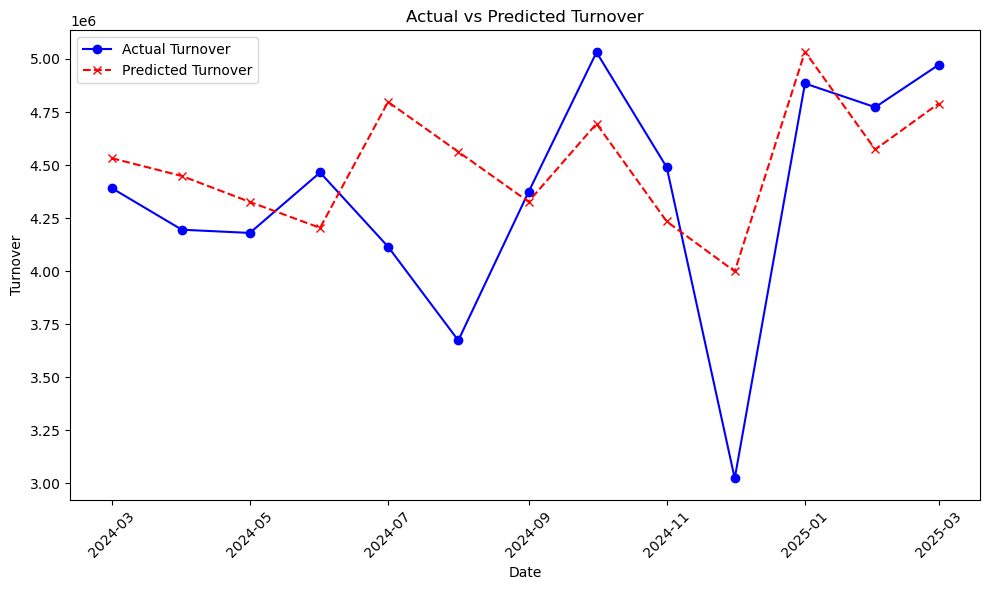
\includegraphics[width=1\linewidth]{images/Linear_Grafiek}
    \caption{Grafiek van het lineaire regressie model}
    \label{fig:GrafiekLinear}
\end{figure}

\begin{figure}[H]
    \centering
    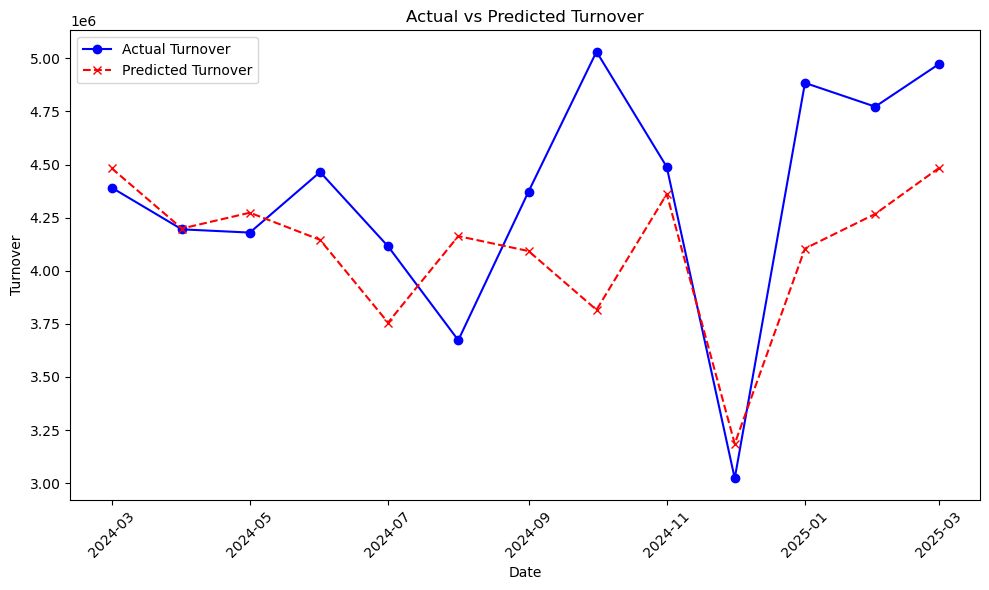
\includegraphics[width=1\linewidth]{images/RandomForrest_Grafiek}
    \caption{Grafiek van het Random Forrest model}
    \label{fig:GrafiekForrest}
\end{figure}

\begin{figure}[H]
    \centering
    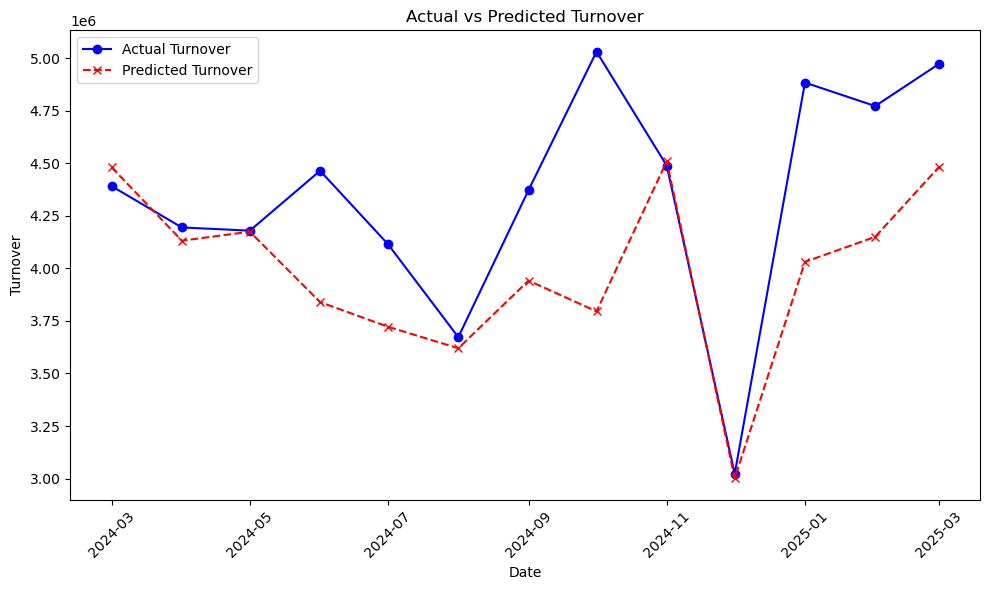
\includegraphics[width=1\linewidth]{images/XGBoost_Grafiek}
    \caption{Grafiek van het XGBoost model}
    \label{fig:GrafiekXGBoost}
\end{figure}

\begin{figure}[H]
    \centering
    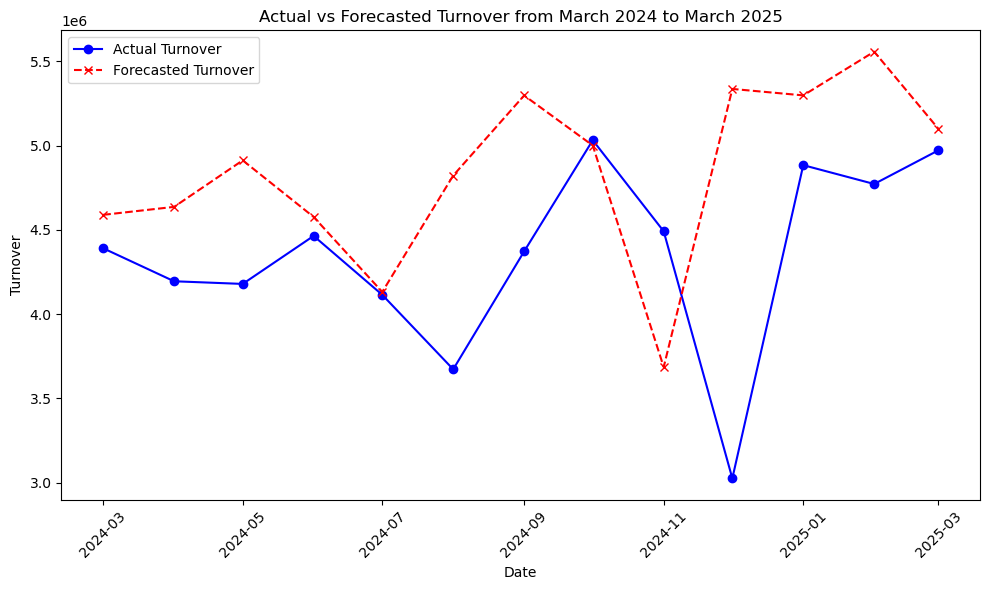
\includegraphics[width=1\linewidth]{images/Samira/Samiragrafiek}
    \caption{Grafiek van het SAMIRA model}
    \label{fig:GrafiekSAMIRA}
\end{figure}

\subsection{Conclusie}

Op basis van de evaluatie van de verschillende modellen blijkt dat lineaire regressie de beste prestaties levert op alle foutmaten (MSE, RMSE en MAE). Hoewel complexere modellen zoals Random Forest en XGBoost vaak betere resultaten kunnen opleveren bij niet-lineaire patronen, bleek lineaire regressie in dit geval het meest geschikt voor deze dataset.

\vspace{1em} 

Daarnaast presteert het SARIMA-model duidelijk slechter dan de andere modellen. Hoewel tijdreeksmodellen zoals SARIMA vaak geschikt zijn voor het modelleren van seizoensgebonden trends en patronen, bleek het in deze situatie minder accuraat bij het voorspellen van de maandelijkse verkoopcijfers.


\newpage

\section{Klantsegmentatie model}

In deze fase van de POC worden verschillende segmentatiemodellen toegepast om klanten te groeperen op basis van hun aankoopgedrag en kenmerken. Er wordt gewerkt met modellen zoals K-Means, DBSCAN, Gaussian Mixture Models (GMM) en K-Modes, die ook categorische klant- en artikeldata meenemen. De clusterdata wordt opgeslagen voor later gebruik in de volgende fase, waarin deze geïntegreerd zal worden met het best presterende salesvoorspellingsalgoritme zonder segmentatie, om te bepalen welk segmentatiemodel de salesvoorspellingen het beste verbetert.

\subsection{Data}

Voor de segmentatiemodellen K-Means, DBSCAN en GMM worden numerieke gegevens gebruikt, zoals totaal gespendeerd bedrag en gemiddeld factuurbedrag. Deze gegevens zijn geschikt voor het identificeren van clusters op basis van het aankoopgedrag van klanten.

\vspace{1em} 

Voor het K-Modes model worden categorische gegevens gebruikt, zoals Customer group, Activity, Competence center en Product type, die inzicht bieden in klantsegmenten op basis van niet-numerieke kenmerken.

\subsection*{Inzicht in de Data}

Deze grafiek toont het totaal gespendeerd bedrag per klant. Het biedt een eerste kijk op het koopgedrag van klanten en helpt om een beter begrip te krijgen van de variatie in uitgaven voordat we de segmentatiemodellen toepassen.

\begin{figure}[H]
    \centering
    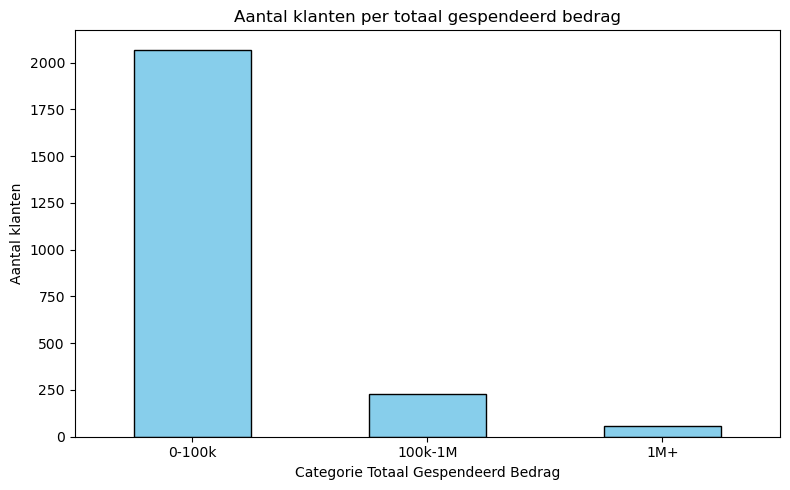
\includegraphics[width=0.8\linewidth]{images/Kmeans/KlantenAnalyse}
    \caption{Klanten per aankoopgroep}
    \label{fig:KlantenPerGroep}
\end{figure}



\subsection{Imports}

\subsection*{Imports voor numerieke segmentatiemodellen}

In deze sectie worden de specifieke bibliotheken geïmporteerd die nodig zijn voor het trainen en evalueren van de numerieke segmentatiemodellen, zoals K-Means, DBSCAN, en Gaussian Mixture Models (GMM). Deze modellen werken met numerieke data.

\vspace{1em}

\begin{listing}[H]
    \begin{minted}{python}
        #Algemene Imports
        import pandas as pd
        import matplotlib.pyplot as plt
        import seaborn as sns
        from sklearn.preprocessing import StandardScaler
        from sklearn.decomposition import PCA
        from deltalake import DeltaTable, write_deltalake
        
        #Specifieke imports per model
        from sklearn.mixture import GaussianMixture
        from sklearn.cluster import KMeans
        from sklearn.cluster import DBSCAN
    \end{minted}
    \caption[Imports voor numerieke segmentatiemodellen]{Imports voor K-Means, DBSCAN en Gaussian Mixture Models.}
\end{listing}

\subsection*{Imports voor categorische segmentatiemodel}

In deze sectie worden de specifieke bibliotheken geïmporteerd die nodig zijn voor het trainen van het K-Modes model, dat geschikt is voor categorische gegevens. Dit model wordt gebruikt om klantgroepen te segmenteren op basis van niet-numerieke kenmerken zoals klantgroep, activiteit en producttype.

\vspace{1em}

\begin{listing}[H]
    \begin{minted}{python}
        import pandas as pd
        import matplotlib.pyplot as plt
        import pyarrow as pa
        from kmodes.kmodes import KModes
        from deltalake import DeltaTable, write_deltalake
    \end{minted}
    \caption[Imports voor K-Modes segmentatiemodel]{Imports voor het K-Modes model.}
\end{listing}


\newpage

\subsection{Segmentatiemodellen}

In de volgende secties wordt uitgelegd hoe de klantgroepen zijn gemaakt en wat de uitkomsten daarvan zijn. Per model wordt beschreven hoe de groepen tot stand kwamen, welke soorten klanten er in elke groep zitten en wat we daaruit kunnen afleiden over hun koopgedrag.

\subsection*{K-Means}


Voor K-Means moet het aantal groepen waarin de data wordt opgedeeld, zelf worden bepaald. Een veelgebruikte manier om dit aantal te kiezen, is de Elbow-methode. Bij deze methode wordt gekeken naar hoe de totale variatie binnen de groepen (de WCSS, oftewel de inertie) afneemt naarmate het aantal clusters toeneemt. In het begin zal de variatie sterk afnemen, maar op een gegeven moment zal het verschil kleiner worden. Het punt waarop deze afname afvlakt, wordt vaak gekozen als het beste aantal clusters. Dit punt wordt het "knikpunt" genoemd.

\vspace{1em}

In de onderstaande grafiek is te zien hoe de WCSS zich gedraagt bij verschillende aantallen clusters. In dit geval is het optimale aantal clusters 3, omdat daar het knikpunt zichtbaar is, wat lijkt op een "elboog".

\begin{figure}[H]
    \centering
    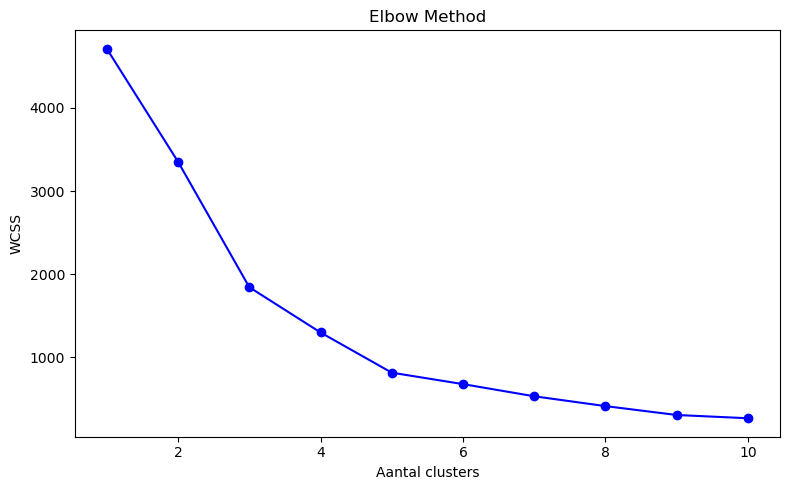
\includegraphics[width=1\linewidth]{images/Kmeans/ElbowMethodKmeans}
    \caption{Elbow method K-means grafiek}
    \label{fig:ElbowMethodKmeans}
\end{figure}


\newpage

\subsection*{K-Modes}

K-Modes is een clusteringtechniek die speciaal ontworpen is voor categorische data. In tegenstelling tot K-Means, dat werkt met numerieke waarden en gebruikmaakt van gemiddelden, bepaalt K-Modes de modus (meest voorkomende waarde) binnen elke groep. Deze methode maakt het mogelijk om categorieën op een logische manier te groeperen zonder dat numerieke afstandsmetingen nodig zijn.

\vspace{1em}

Ook bij K-Modes moet het aantal clusters vooraf worden bepaald. Hiervoor kan een aangepaste versie van de Elbow-methode worden gebruikt, waarbij de kosten (bijvoorbeeld het aantal niet-overeenkomende categorieën binnen clusters) worden geanalyseerd. Het optimale aantal clusters wordt gekozen op het punt waar het toevoegen van extra clusters nauwelijks nog zorgt voor een verdere afname van de kosten.

\vspace{1em}

In de onderstaande grafiek is te zien hoe de kosten zich gedragen bij verschillende aantallen clusters. Het optimale aantal clusters is , omdat hier de afname in kosten aanzienlijk kleiner wordt en verder verhogen van het aantal clusters nauwelijks nog tot een verbetering leidt.


\begin{figure}[H]
    \centering
    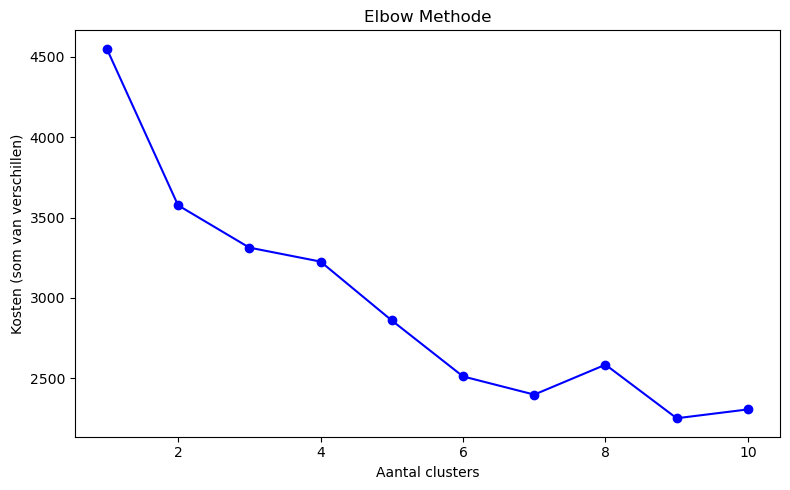
\includegraphics[width=1\linewidth]{images/Kmodes/ElbowmethodKmodes}
    \caption{Elbow method K-modes grafiek}
    \label{fig:ElbowMethodKmodes}
\end{figure}

\newpage

\subsection*{DBSCAN}

Met DBSCAN wordt het aantal clusters automatisch bepaald op basis van de dichtheid van de data. Hierbij worden punten die niet aan de dichtheidscriteria voldoen als outliers (-1) gemarkeerd, terwijl de overige punten in clusters worden ingedeeld. Het aantal clusters wordt dus dynamisch berekend, zonder vooraf gedefinieerde grenzen.

\subsection*{GMM}

Bij GMM wordt het aantal clusters automatisch bepaald door de data te modelleren als een combinatie van meerdere Gaussian distributies. In tegenstelling tot DBSCAN, dat zich richt op dichtheid, gebruikt GMM statistische verdelingen om de optimale clustering van de gegevens te berekenen.

\newpage

\subsection{Resultaten}

Alle clusterdata van elk segmentatiemodel is weggeschreven naar een Lakehouse voor gebruik in fase 5.

\subsection*{Numerieke segmentatiemodellen}

Voor de numerieke segmentatie modellen zijn er drie grafieken gekozen om de prestaties van de clusteringstechnieken te analyseren. Deze grafieken geven inzicht in verschillende aspecten van de clusters en hoe de klanten zijn verdeeld over de verschillende groepen.

\vspace{1em}

De eerste grafiek biedt een visuele weergave van de clusters in een 2D-ruimte. Hierbij worden de eerste twee hoofdcomponenten (bijvoorbeeld PCA1 en PCA2) gebruikt om de klanten te plotten, waarbij elke kleur een cluster vertegenwoordigt.Voor K-Means worden de centroids van de clusters gemarkeerd met een "X", die de centrale punten van de klantgroepen aanduiden. Deze grafiek biedt een overzicht van de verdeling van de klanten over de clusters en toont de centrale punten van elke groep.

\vspace{1em}

De tweede grafiek toont het aantal klanten per cluster. Elke balk in de grafiek representeert het aantal klanten binnen een specifiek cluster. De x-as geeft de clusters weer, terwijl de y-as het aantal klanten binnen elk cluster toont. Deze grafiek maakt het mogelijk om te zien hoe de klanten zijn verdeeld over de clusters en helpt om te begrijpen welke groepen groter of kleiner zijn.

\vspace{1em}

De derde grafiek biedt inzicht in het verband tussen twee variabelen, namelijk het gemiddelde factuurbedrag en het totaal uitgegeven bedrag per klant, opgedeeld per cluster. Op de x-as staat het gemiddelde factuurbedrag per klant, terwijl de y-as het totaal bedrag toont dat een klant heeft uitgegeven. Elke kleur in de grafiek komt overeen met een cluster, waardoor het duidelijk wordt hoe de verschillende klantgroepen zich verhouden op basis van deze twee variabelen.


\subsection*{K-means}

\begin{figure}[H]
    \centering
    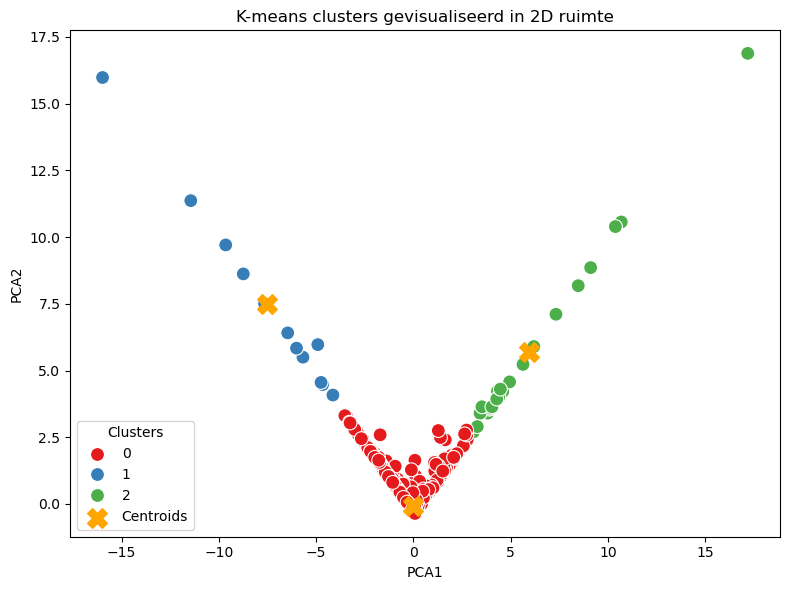
\includegraphics[width=0.8\linewidth]{images/Kmeans/2DrepresentatieKmeans}
    \caption{2D-representatie van de K-Means clusters met PCA en centroids}
    \label{fig:PCA_KMeans}
\end{figure}

\begin{figure}[H]
    \centering
    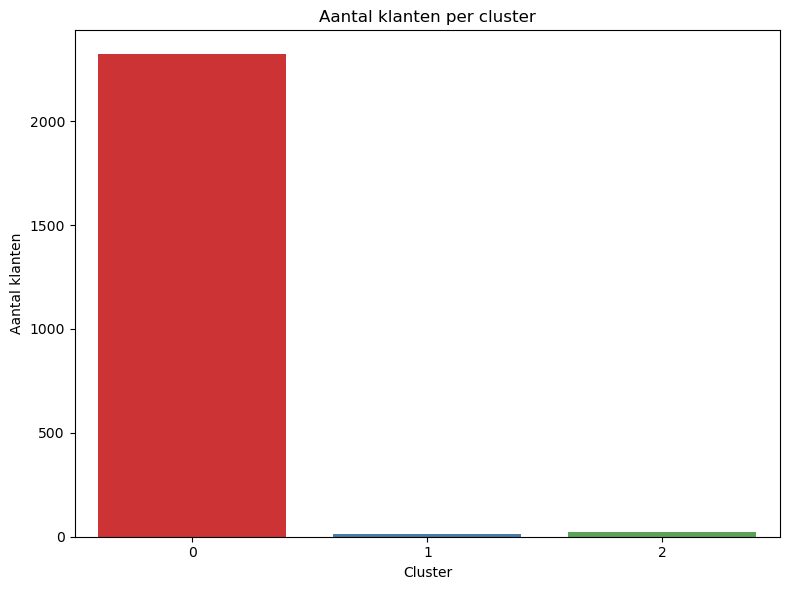
\includegraphics[width=0.8\linewidth]{images/Kmeans/AantalKlantenKMeans}
    \caption{Aantal klanten per cluster (K-Means)}
    \label{fig:Klanten_KMeans}
\end{figure}

\begin{figure}[H]
    \centering
    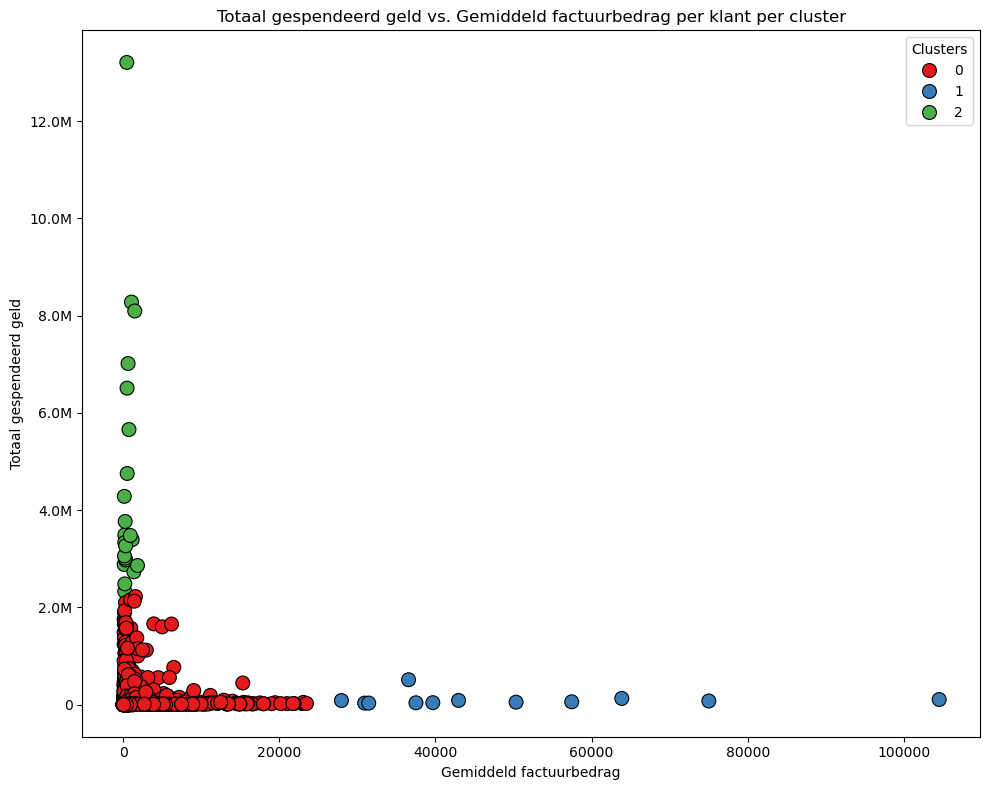
\includegraphics[width=0.8\linewidth]{images/Kmeans/KMeansClusterAnalyse}
    \caption{Analyse van gemiddelde factuurbedrag vs. totaal gespendeerd bedrag per klant (K-Means)}
    \label{fig:Analyse_KMeans}
\end{figure}

\subsection*{GMM}

\begin{figure}[H]
    \centering
    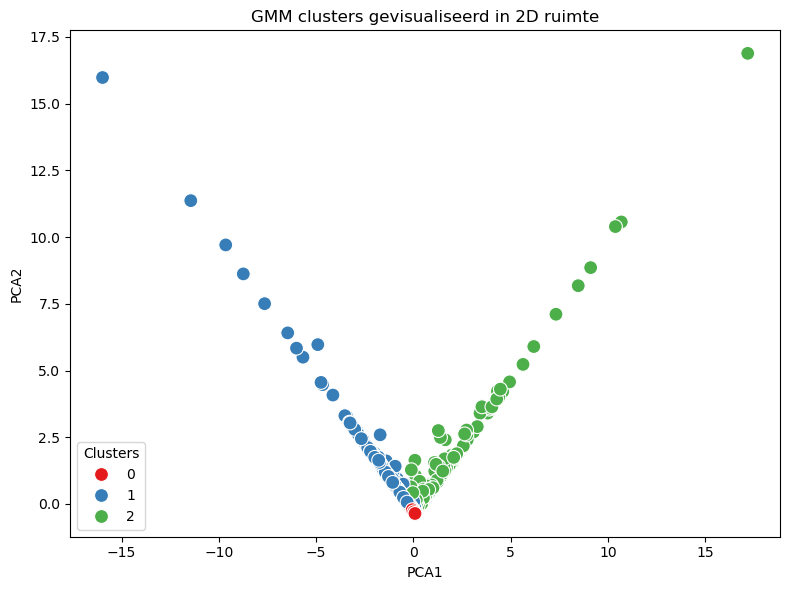
\includegraphics[width=0.8\linewidth]{images/GMM/AnalyseGMM}
    \caption{2D-representatie van de GMM clusters met PCA}
    \label{fig:PCA_GMM}
\end{figure}

\begin{figure}[H]
    \centering
    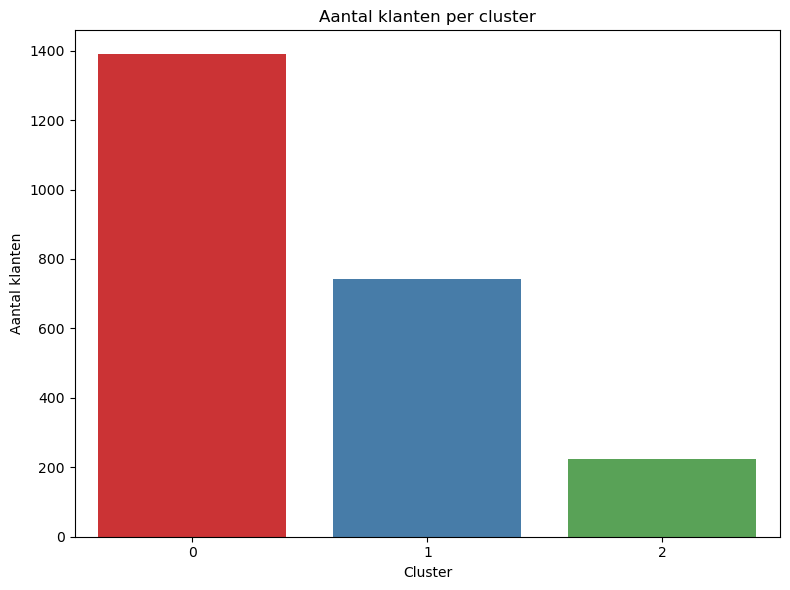
\includegraphics[width=0.8\linewidth]{images/GMM/AantalKlantenGMM}
    \caption{Aantal klanten per cluster (GMM)}
    \label{fig:Klanten_GMM}
\end{figure}

\begin{figure}[H]
    \centering
    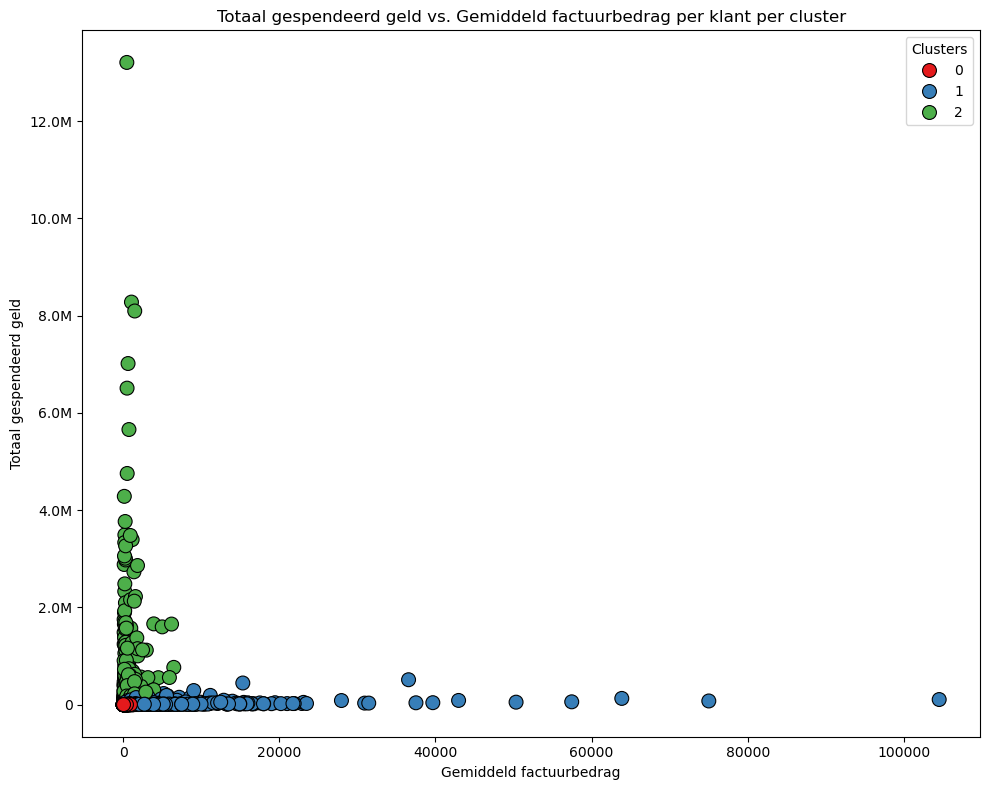
\includegraphics[width=0.8\linewidth]{images/GMM/Analyse2GMM}
    \caption{Analyse van gemiddelde factuurbedrag vs. totaal gespendeerd bedrag per klant (GMM)}
    \label{fig:Analyse_GMM}
\end{figure}

\subsection*{DBSCAN}

\begin{figure}[H]
    \centering
    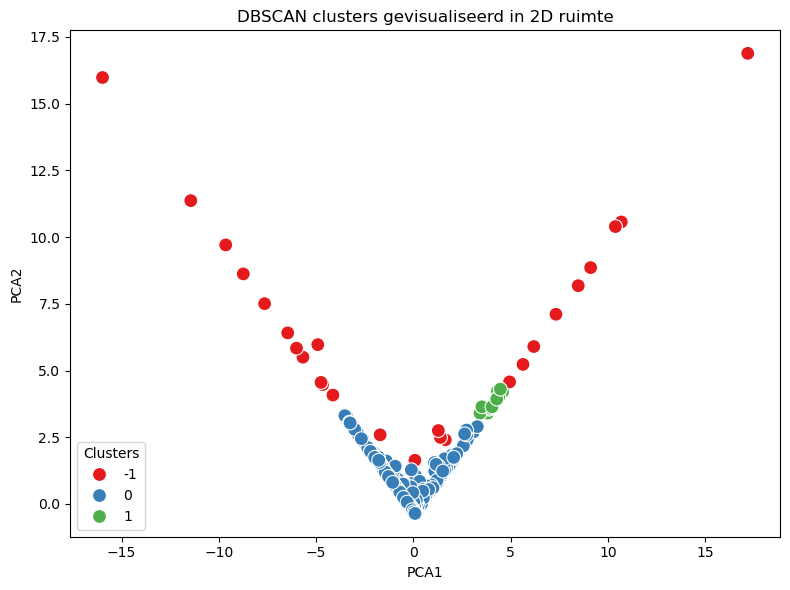
\includegraphics[width=0.8\linewidth]{images/DBSCAN/AnalyseDBSCAN}
    \caption{2D-representatie van de DBSCAN clusters met PCA}
    \label{fig:PCA_DBSCAN}
\end{figure}

\begin{figure}[H]
    \centering
    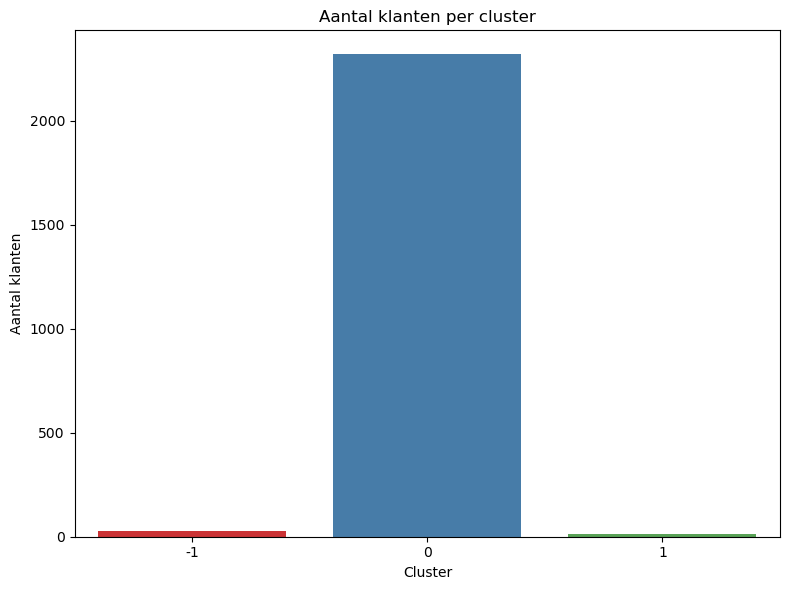
\includegraphics[width=0.8\linewidth]{images/DBSCAN/AantalKlantenDBSCAN}
    \caption{Aantal klanten per cluster (DBSCAN)}
    \label{fig:Klanten_DBSCAN}
\end{figure}

\begin{figure}[H]
    \centering
    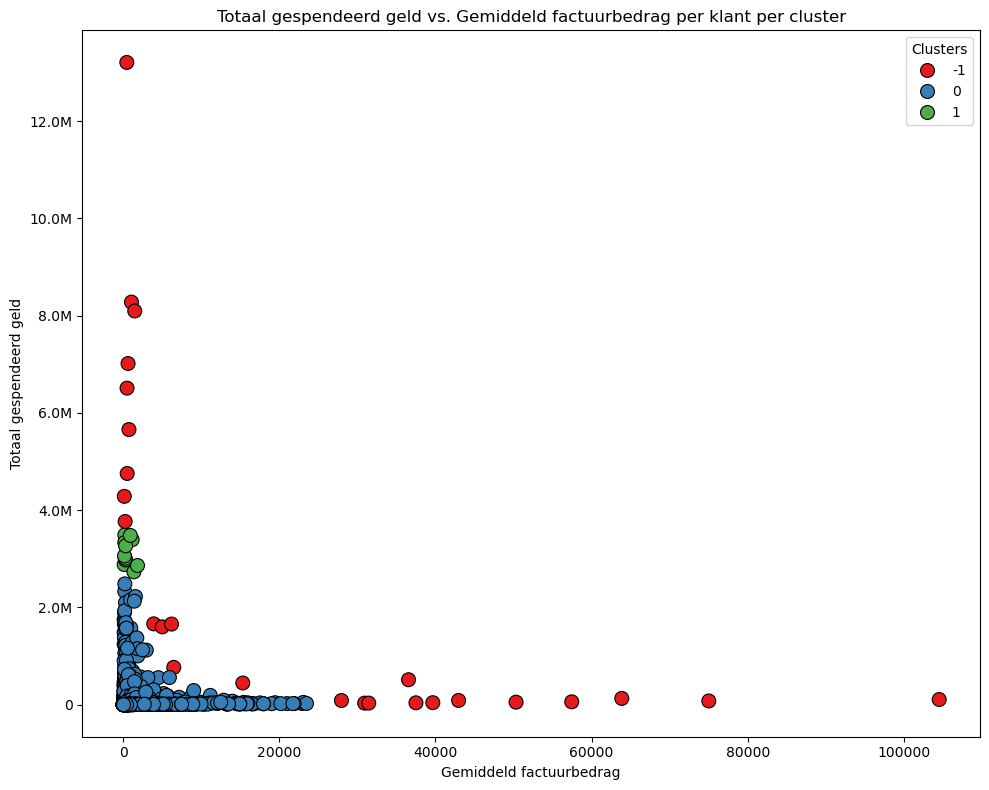
\includegraphics[width=0.8\linewidth]{images/DBSCAN/Analyse2DBSCAN}
    \caption{Analyse van gemiddelde factuurbedrag vs. totaal gespendeerd bedrag per klant (DBSCAN)}
    \label{fig:Analyse_DBSCAN}
\end{figure}


\subsection*{Categorisch segmentatiemodel}

Voor de categorische data kunnen de clusters niet altijd op dezelfde manier worden geanalyseerd als bij de numerieke segmentatiemodellen. Daarom wordt er gebruik gemaakt van andere grafieken en tabellen om inzicht te krijgen in de verdeling van klanten binnen de clusters.

\vspace{1em}

De eerste grafiek toont het aantal klanten per cluster, waarbij de x-as de clusters weergeeft en de y-as het aantal klanten per cluster. Deze grafiek biedt inzicht in hoe de klanten verdeeld zijn over de verschillende clusters.

\vspace{1em}

Naast de grafiek, wordt er ook een tabel gepresenteerd die de meest voorkomende waarden voor elk categorisch kenmerk binnen elk cluster weergeeft. Dit biedt een gedetailleerder overzicht van de segmentatie, waarbij de meest representatieve klantkenmerken voor elk cluster worden getoond. De tabel bevat bijvoorbeeld de meest voorkomende klantgroep, activiteit, competentiecentrum en producttype per cluster. Dit helpt bij het begrijpen van de klantprofielen die zich in de verschillende segmenten bevinden.


\begin{figure}[H]
    \centering
    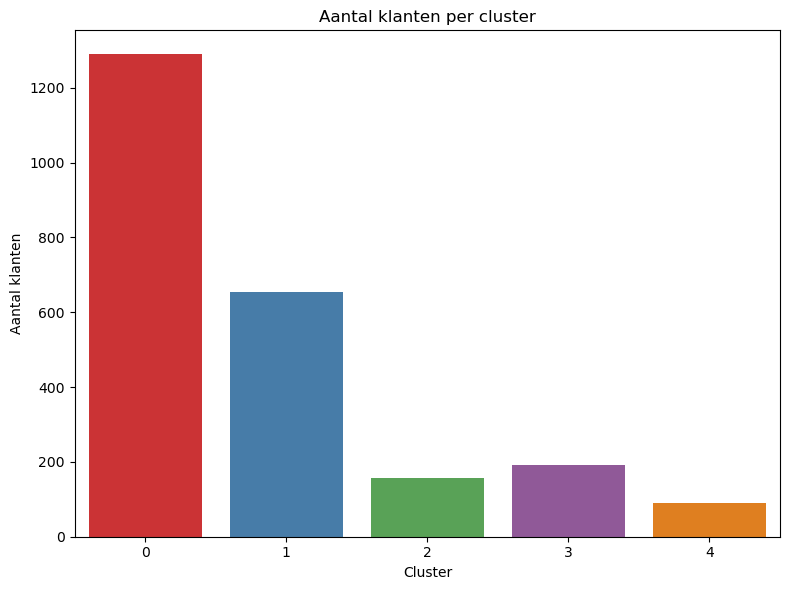
\includegraphics[width=1\linewidth]{images/Kmodes/AantalKlantenCluster}
    \caption{Aantal klanten per cluster (K-Modes))}
    \label{fig:KlantenK-Modes}
\end{figure}


\begin{table}[H]
    \centering
    \begin{tabular}{|c|c|c|c|c|c|}
        \hline
        \textbf{Cluster} & \textbf{Klantgroep} & \textbf{Activiteit} & \textbf{Competentiecentrum} & \textbf{Producttype} & \textbf{Aantal Klanten} \\
        \hline
        0 & Overige & Trading & Unknown & Unknown & 1289 \\
        1 & Utiliteit & Trading & Thermal insulation & Board / sheets & 653 \\
        2 & Installateur & Trading & Accessories & Unknown & 90 \\
        3 & Utiliteit & Trading & Acoustic insulation & Unknown & 193 \\
        4 & OEM & Trading & Thermal insulation & Unknown & 158 \\
        \hline
    \end{tabular}
    \caption{Aantal klanten per cluster op basis van K-Modes centroiden}
    \label{tab:AantalKlantenPerClusterCategorie}
\end{table}

\subsection{Conclussie}

De uiteindelijke beoordeling van de effectiviteit van de segmentatiemodellen wordt in de volgende fase uitgevoerd, wanneer de invloed van de segmentatie op de nauwkeurigheid van het regressiemodel kan worden geanalyseerd. In deze fase worden de trends van elk model kort besproken.

\subsection*{K-Means}

Met K-Means is er een duidelijk patroon te herkennen. Groep 0 bevat de grootste hoeveelheid klanten en kan worden beschouwd als de algemene groep. Groep 1 omvat klanten met een hoog gemiddeld factuurbedrag, maar een lage totaal besteding. Ten slotte bevat groep 2 klanten met een laag gemiddeld factuurbedrag, maar een hoge totale besteding.


\subsection*{GMM}

Bij GMM zijn er vergelijkbare patronen als bij K-Means. Groep 0 bevat klanten met zowel een laag totaal besteed bedrag als een laag gemiddeld factuurbedrag. Groep 1 omvat klanten met een hoog gemiddeld factuurbedrag en een laag totaal besteed bedrag. Ten slotte heeft groep 2 klanten met een hoog totaal besteed bedrag, maar een laag gemiddeld factuurbedrag. Wat opvalt bij GMM is dat de groepen minder geneigd zijn om alleen de outliers te bevatten, maar in plaats daarvan meer klanten opnemen, waardoor elke groep breder vertegenwoordigd is.

\subsection*{DBSCAN}

Bij DBScan is het anders. Er is één algemene groep, groep 0, die een grote hoeveelheid klanten bevat. Deze groep vertoont veel variatie in zowel het totaal besteed bedrag als het gemiddelde factuurbedrag, wat betekent dat zowel klanten met lage als hoge bestedingen en factuurbedragen in deze groep vallen. Vervolgens is er groep 1, die klanten omvat die tussen de 3 miljoen en 3,75 miljoen hebben besteed, met een laag gemiddeld factuurbedrag. Ten slotte zijn er de outliers volgens DBScan, die als groep -1 worden geclassificeerd. Deze klanten hebben aan de ene kant een hoge totaal besteed bedrag en een laag gemiddeld factuurbedrag, terwijl aan de andere kant klanten met een hoog gemiddeld factuurbedrag en een laag totaal besteed bedrag vallen. Daarnaast zijn er ook enkele klanten die een beetje buiten de algemene groep vallen.

\newpage

\subsection*{K-Modes}

Bij K-Modes clustering zijn vijf klantgroepen gevormd op basis van categorische kenmerken zoals klantgroep, activiteit, competentiecentrum en producttype. Het aantal clusters is vooraf bepaald op vijf.

\vspace{1em}

Groep 0 is de grootste en bestaat voornamelijk uit klanten die onder "Overige" vallen. Bij veel van deze klanten zijn de gegevens over het competentiecentrum en producttype niet bekend. Het lijkt vooral een restgroep te zijn voor klanten die moeilijk in een andere groep te plaatsen zijn of waarvan de gegevens onvolledig zijn.

\vspace{1em}

Groep 1 bestaat vooral uit klanten in de klantgroep "Utiliteit", die zich richten op thermische isolatie. Zij kopen vooral producten uit de categorie "Board / sheets". Deze groep heeft een duidelijk profiel en is goed te onderscheiden van de andere groepen.

\vspace{1em}

Groep 2 is de kleinste groep en bestaat voornamelijk uit "Installateurs", die vooral accessoires als competentie centrum hebben. De beperkte grootte van deze groep wijst erop dat het om een meer gespecialiseerde niche gaat binnen de klantengroep.

\vspace{1em}

Groep 3 bevat opnieuw klanten uit de "Utiliteit", maar in dit geval richten ze zich op akoestische isolatie. Dit laat zien dat er binnen dezelfde klantgroep duidelijke verschillen zijn in voorkeur en focus, zoals het onderscheid tussen thermische en akoestische isolatie.

\vspace{1em}

Groep 4 bestaat uit OEM-klanten, die ook actief zijn in thermische isolatie. Het producttype is bij deze groep vaak onbekend, maar ze vormen een aparte groep met een eigen profiel, dat vooral bepaald wordt door hun klanttype.

\vspace{1em}

De verdeling van de klanten over deze clusters en hun specifieke kenmerken zijn te zien in Tabel~\ref{tab:AantalKlantenPerClusterCategorie}.

\newpage

\section{Regressiemodellen met klantsegmentatie}

In deze fase van de Proof of Concept (POC) wordt een combinatie gemaakt van de regressiemodellen uit Fase 3 en de segmentatiemodellen uit Fase 4. Het doel is om te analyseren welk regressiemodel het meest verbetert door de klantsegmentatie. Elk regressiemodel dat in Fase 3 is ontwikkeld, wordt gecombineerd met de segmentatiemodellen die in Fase 4 zijn gemaakt, en de prestaties van de modellen worden vervolgens geëvalueerd.

\subsection{Code en Implementatie}

Voor de implementatie van de regressiemodellen met klantsegmentatie is dezelfde code en dezelfde imports gebruikt als in Fase 3. Het enige verschil is dat de clusters, die uit de segmentatiemodellen in Fase 4 komen, aan de dataset zijn toegevoegd. Dit wordt gedaan door de klantsegmentatie per maand te koppelen aan de regressievoorspellingen.

\vspace{1em}

In plaats van enkel de turnover per jaar-maand te voorspellen, wordt de turnover nu gesplitst per cluster binnen dezelfde jaar-maand. Voor iedere maand wordt de turnover per cluster voorspeld. Vervolgens worden de voorspellingen per cluster gecombineerd om de uiteindelijke voorspellingen per maand te verkrijgen. Dit maakt het mogelijk om de prestaties van het model per cluster te evalueren en de MSE, MAE en RMSE te vergelijken, zoals te zien is in Tabel~\ref{tab:model_evaluation}, zodat geanalyseerd kan worden in hoeverre klantsegmentatie de voorspellingen verbetert.

\vspace{1em}

Voor K-Means werd ervoor gekozen om zowel de resultaten met drie clusters als met twee clusters te evalueren. De motivatie hiervoor is dat bij het gebruik van drie clusters, groep 1 zeer weinig datapunten bevatte. Dit werd ondervonden tijdens het programmeren van de combinatie van Linear Regression en K-Means, toen de maatstaven onverwacht hoog terugkwamen. Het bleek dat K-Means met drie clusters niet optimaal was voor het bereiken van nauwkeurige voorspellingen.

In de aangepaste versie werden de datapunten uit de inconsistente cluster samengevoegd met de grootste cluster.

\subsection{Resultaten}

In deze sectie worden de resultaten gepresenteerd voor alle regressiemodellen in combinatie met de verschillende segmentatiemodellen. De prestaties worden geëvalueerd aan de hand van drie standaardcriteria: MAE, RMSE en MSE. Daarbij wordt een overzichtstabel opgesteld met de segmentatiemodellen per regressiemodel. Daarnaast wordt per segmentatiemodel een grafiek getoond die de voorspelde en de werkelijke omzet met elkaar vergelijkt.


\subsection*{Lineaire Regressie}

Uit de evaluatie van de lineaire regressie in combinatie met de verschillende segmentatiemodellen blijkt dat geen enkel segmentatiemodel een positief effect heeft op de prestaties. Alleen K-Means met twee clusters komt dicht bij het oorspronkelijke model, maar dit resulteert nog steeds niet in een verbetering van de modelprestaties.

\vspace{1em}

Hieruit kunnen we dus concluderen dat lineaire regressie geen verbeteringen oplevert voor de precisie van het model in combinatie met de segmentatiemodellen.

\begin{table}[H]
    \centering
    \caption{Evaluatie van Segmentatiemodellen (Lineare Regressie)}
    \label{tab:segmentation_model_evaluation}
    \begin{tabular}{|l|r|r|r|}
        \hline
        \textbf{Segmentatiemodel} & \textbf{MSE} & \textbf{RMSE} & \textbf{MAE} \\ \hline
        Geen Segmentatie         & 202,982,205,716 & 450,535 & 346,951  \\ \hline
        DBSCAN                   & 203,660,022,011 & 451,287 & 366,047 \\ \hline
        GMM                      & 213,496,413,842 & 462,057 & 359,523 \\ \hline
        K-Means                  & 1,564,135,315,178 & 1,250,654 & 1,105,220 \\ \hline
        K-Means (2 clusters)     & 202,987,515,188 & 450,541 & 346,944 \\ \hline
        K-Modes                  & 235,814,056,435 & 485,607 & 375,252 \\ \hline
    \end{tabular}
\end{table}

\subsection*{Random Forest}

Met Random Forest zien we een duidelijke verbetering bij het gebruik van elk segmentatiemodel in vergelijking met het model zonder segmentatie. De twee beste segmentatiemodellen zijn GMM en K-Means (2 clusters), die beide beter presteren dan de andere modellen. Het valt op dat de MAE voor GMM lager is dan voor K-Means (2 clusters), wat betekent dat er minder kleine afwijkingen zijn in de voorspellingen. Aan de andere kant heeft K-Means (2 clusters) een lagere RMSE, wat erop wijst dat de voorspellingen dichter bij de werkelijke waarden liggen, met minder extreme afwijkingen.



\begin{table}[H]
    \centering
    \caption{Evaluatie van Segmentatiemodellen (Random Forest}
    \label{tab:rf_segmentation_model_evaluation}
    \begin{tabular}{|l|r|r|r|}
        \hline
        \textbf{Segmentatiemodel} & \textbf{MSE} & \textbf{RMSE} & \textbf{MAE} \\ \hline
        Geen Segmentatie         & 242,022,929,294 & 491,598 & 378,430 \\ \hline
        DBSCAN                   & 195,606,503,305 & 442,274 & 354,030 \\ \hline
        GMM                      & 181,570,304,039 & 426,111 & 323,223 \\ \hline
        K-Means                  & 191,538,053,557 & 437,651 & 348,390 \\ \hline
        K-Means (2 clusters)     & 173,878,934,037 & 416,988 & 331,119 \\ \hline
        K-Modes                  & 197,406,370,649 & 444,304 & 342,233 \\ \hline
    \end{tabular}
\end{table}

\subsection*{XGBoost}

Met XGBoost zien we een verbetering bij het gebruik van elk segmentatiemodel in vergelijking met het model zonder segmentatie. De twee segmentatiemodellen die het beste presteren zijn DBSCAN en GMM. DBSCAN heeft een lagere RMSE, wat aangeeft dat het model minder zware uitbijters bevat, terwijl GMM een lagere MAE heeft, wat duidt op minder kleine afwijkingen in de voorspellingen. 

\begin{table}[H]
    \centering
    \caption{Evaluatie van Segmentatiemodellen (XGBoost)}
    \label{tab:segmentation_model_evaluation_xgboost}
    \begin{tabular}{|l|r|r|r|}
        \hline
        \textbf{Segmentatiemodel} & \textbf{MSE} & \textbf{RMSE} & \textbf{MAE} \\ \hline
        Geen Segmentatie         & 282,605,525,485 & 531,607 & 376,649 \\ \hline
        DBSCAN                   & 198,351,735,089 & 445,367 & 331,881 \\ \hline
        GMM                      & 212,792,775,817 & 461,295 & 328,150 \\ \hline
        K-Means                  & 201,899,764,153 & 449,333 & 342,673 \\ \hline
        K-Means (2 clusters)     & 222,381,530,790 & 471,573 & 369,660 \\ \hline
        K-Modes                  & 219,390,746,160 & 468,392 & 359,734 \\ \hline
    \end{tabular}
\end{table}


\subsection*{Conclusie}

Zonder segmentatie was het beste model lineaire regressie. Dit was ook het enige regressiemodel dat geen verbeteringen zag met het gebruik van segmentatie. Na het integreren van segmentatie presteerden alle XGBoost en Random Forest-modellen beter dan het lineaire regressiemodel zonder segmentatie.

\vspace{1em}

De beste combinatie hierin was Random Forest met K-Means (2 clusters) voor RMSE en MSE, en Random Forest met GMM voor MAE. Deze bevinding toont aan dat segmentatie in combinatie met de juiste modelkeuze leidt tot verbeterde prestaties.

\newpage

\subsection{Resultaten Segmentatiemodellen}

In deze sectie worden de prestaties van de verschillende segmentatiemodellen geëvalueerd in combinatie met de regressiemodellen, buiten lineaire regressie aangezien hier geen enkele verbetering is opgetreden door de segmentatie. De impact van de segmentatie op de modelnauwkeurigheid wordt geanalyseerd aan de hand van de maatstaven. Elk segmentatiemodel wordt afzonderlijk beoordeeld om te begrijpen hoe de segmentatie de prestaties van de regressiemodellen beïnvloedt.


\subsection*{DBScan}

DBSCAN toont bij beide regressiemodellen een duidelijke verbetering in de maatstaven vergeleken met het model zonder segmentatie. In combinatie met XGBoost levert DBSCAN de beste resultaten voor zowel RMSE als MSE, en het tweede beste resultaat voor MAE. Echter, bij het gebruik van het Random Forest-model behaalt DBSCAN de voorlaatste positie, achter K-Means voor zowel RMSE als MSE, en behaalt het de hoogste MAE.

\vspace{1em}

Hieruit kan afgeleid worden dat DBSCAN goed samenwerkt met XGBoost maar niet met Random Forest.

\subsection*{GMM}

GMM toont bij beide regressiemodellen een duidelijke verbetering in de maatstaven vergeleken met het model zonder segmentatie. Bij Random Forest behaalt GMM de beste MAE en de tweede beste RMSE en MSE. Bij XGBoost levert GMM opnieuw de beste MAE, maar behaalt het de derde plaats voor zowel RMSE als MSE.

\vspace{1em}

Hieruit kan worden afgeleid dat GMM effectief is in het verminderen van kleine fouten, maar niet het beste model is om zware uitbijters te verkleinen. Daarnaast blijkt GMM goed samen te werken met zowel XGBoost als Random Forest.

\newpage

\subsection*{K-Means}

Voor K-Means en K-means (2 clusters) zien we een duidelijke verbetering in de maatstaven vergeleken met het model zonder segmentatie.

\subsubsection*{K-Means}

Bij Random Forest is de verbetering voor K-Means minder significant in vergelijking met de andere modellen, met de derde hoogste MSE en RMSE, en de op één na hoogste MAE. Bij XGBoost presteert K-Means beter, waar het de tweede beste RMSE en MSE oplevert, en het derde beste MAE.

\vspace{1em}

Hieruit kan worden geconcludeerd dat K-Means beter presteert in combinatie met XGBoost dan met Random Forest. Hoewel K-Means in beide gevallen beter scoort dan het model zonder segmentatie, hoort het over het algemeen niet bij de sterkste segmentatiemodellen in deze analyse.


\subsubsection*{K-Means (2 clusters)}

K-Means (2 clusters) behaalt de beste RMSE en MSE in combinatie met Random Forest en scoort daar ook de tweede beste MAE. In combinatie met XGBoost zijn de resultaten echter aanzienlijk minder, met de slechtste RMSE en MAE van alle segmentatiemodellen.

\vspace{1em}

Hieruit kunnen we concluderen dat K-Means (2 clusters) vooral goed presteert in combinatie met Random Forest, maar duidelijk minder effectief is in combinatie met XGBoost.


\subsection*{K-Modes}

Voor K-Modes zien we een duidelijke verbetering in de maatstaven vergeleken met het model zonder segmentatie. Met Random Forest heeft K-Modes de hoogste RMSE en MSE en de derde hoogste MAE, terwijl het bij XGBoost de tweede slechtste RMSE en tweede slechtste MAE behaalt.

\vspace{1em}

Hieruit kan besloten worden dat K-Modes, als enig categorisch segmentatiemodel, minder goed presteerde in vergelijking met de andere segmentatiemodellen.

\newpage

\subsection*{Conclusie}


Gezien het gebruik van twee verschillende regressiemodellen, Random Forest en XGBoost, zijn aparte rangschikkingen opgesteld om de beste segmentatiemodellen te evalueren. De rangschikkingen zijn opgesplitst op basis van de twee maatstaven: RMSE en MAE. Deze splitsing is noodzakelijk omdat de keuze tussen deze twee afhankelijk is van de specifieke doelstellingen van het model. RMSE is gevoeliger voor grotere afwijkingen en is nuttig wanneer het minimaliseren van deze van belang is. MAE daarentegen biedt een meer gebalanceerde benadering, waarbij de gemiddelde afwijking per voorspelling wordt benadrukt, wat geschikt is voor situaties waarin kleinere afwijkingen belangrijker zijn.

\vspace{1em}

Uit de resultaten blijkt dat, voor het minimaliseren van grote afwijkingen, K-Means (2 clusters) het beste presteert voor Random Forest, terwijl DBSCAN het beste presteert voor XGBoost. Voor het minimaliseren van kleinere afwijkingen blijkt het GMM-model de beste keuze te zijn voor zowel Random Forest als XGBoost.



\begin{table}[H]
    \centering
    \caption{Evaluatie van segmentatiemodellen (Random Forest) - Rangschikking op RMSE en MAE}
    \label{tab:rf_segmentation_model_evaluation_combined}
    \begin{tabular}{|l|l|r|l|r|}
        \hline
        \textbf{Rang} & \textbf{Model (RMSE)} & \textbf{RMSE} & \textbf{Model (MAE)} & \textbf{MAE} \\ \hline
        1 & K-Means (2 clusters)     & 416,988 & GMM                      & 323,223 \\ \hline
        2 & GMM                      & 426,111 & K-Means (2 clusters)     & 331,119 \\ \hline
        3 & K-Means                  & 437,651 & K-Modes                  & 342,233 \\ \hline
        4 & DBSCAN                   & 442,274 & K-Means                  & 348,390 \\ \hline
        5 & K-Modes                  & 444,304 & DBSCAN                   & 354,030 \\ \hline
        6 & Geen Segmentatie         & 491,598 & Geen Segmentatie         & 378,430 \\ \hline
    \end{tabular}
\end{table}

\begin{table}[H]
    \centering
    \caption{Evaluatie van segmentatiemodellen (XGBoost) - Rangschikking op RMSE en MAE}
    \label{tab:segmentation_model_evaluation_xgboost_combined}
    \begin{tabular}{|l|l|r|l|r|}
        \hline
        \textbf{Rang} & \textbf{Model (RMSE)} & \textbf{RMSE} & \textbf{Model (MAE)} & \textbf{MAE} \\ \hline
        1 & DBSCAN                   & 445,367 & GMM                      & 328,150 \\ \hline
        2 & K-Means                  & 449,333 & DBSCAN                   & 331,881 \\ \hline
        3 & GMM                      & 461,295 & K-Means                  & 342,673 \\ \hline
        4 & K-Modes                  & 468,392 & K-Modes                  & 359,734 \\ \hline
        5 & K-Means (2 clusters)     & 471,573 & K-Means (2 clusters)     & 369,660 \\ \hline
        6 & Geen Segmentatie         & 531,607 & Geen Segmentatie         & 376,649 \\ \hline
    \end{tabular}
\end{table}




